%======================================================================@
\chapter{Classes} \label{c:classes}
%======================================================================@

%=======================================================================
\section{\code{Ensemble} classes}
%=======================================================================

The \code{Ensemble} class is used to store a collection of simulations.

% An Ensemble contains an aggregate list of Simulations
% It may contain a single Simulation

\subsection{Attributes.}

\subsection{Operations}


%=======================================================================
\section{\code{Simulation} class}
%=======================================================================

The \code{Simulation} class is used to define a simulation.  

\begin{itemize}
\item \code{Problem}
\item \code{Physics}
\item \code{Method}
\item \code{IO}
\end{itemize}

\subsection{Attributes.}

\subsection{Operations}

%=======================================================================
\section{\code{Parameters} class}
%=======================================================================

The \code{Parameters} class read in a parameter file or files, and
provide the application access to parameter values.


\subsection{Attributes}

\subsection{Operations}

%=======================================================================
\section{\code{Physics} class}
%=======================================================================


\subsection{Attributes}

\subsection{Operations}

%=======================================================================
\section{\code{Domain} class}
%=======================================================================

The \code{Domain} class is related to the \code{Region} class.


\subsection{Attributes}

\subsection{Operations}

%=======================================================================
\section{\code{BC} class}
%=======================================================================

The \code{BC} class defines boundary conditions on a \code{Domain}.



\subsection{Attributes}

\subsection{Operations}

%=======================================================================
\section{\code{IC} class}
%=======================================================================

The \code{IC} class defines initial conditions for a set of
\code{Field}s in a \code{Domain}.


\subsection{Attributes}

\subsection{Operations}

%=======================================================================
\section{\code{Region} classes}
%=======================================================================

The \code{Domain} class is related to the \code{Region} class.


\subsection{Attributes}

\subsection{Operations}

%=======================================================================
\section{\code{Problem} class}
%=======================================================================

The \code{Problem} class defines the problem to be solved, including
the domain, boundary conditions, and initial field values.


\subsection{Attributes}

\subsection{Operations}

%=======================================================================
\section{\code{Field} class} \label{ss:field}
%=======================================================================

A \code{Field} represents a discrete multiresolution scalar or vector
field.  A \code{Field} is associated with a \code{Hierarchy}, and is
composed of \code{Array}'s defined on a subset of \code{Grid}s in the
\code{Hierarchy}.

\subsection{Attributes}

\subsection{Operations}

%=======================================================================
\section{\code{Units} class}
%=======================================================================

A \code{Units} class represents the physical units for the data in a
\code{Field}.

\subsection{Attributes}

\subsection{Operations}

\newpage

%======================================================================@
\chapter{Data Classes} \label{s:data-classes}
%======================================================================@

\centerline{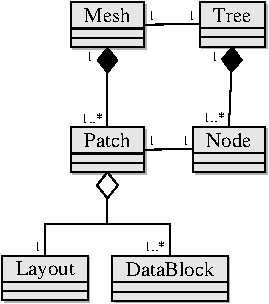
\includegraphics{uml/amr.1}}

%=======================================================================
\section{\code{Hierarchy} class}
%=======================================================================

A \code{Hierarchy} class represents a distributed structured AMR grid
hierarchy.  A \code{Hierarchy} can be considered to be an aggregate of
\code{Level}s, each of which in turn is an aggregate of individual
\code{Patch}es.  A patch is composed of a \code{Box}, which defines
the position and size in space, and some number of \code{Array}s, which
are used to store \code{Field} data (see \S\ref{ss:field}).



\subsection{Attributes}

\subsection{Operations}

%=======================================================================
\section{\code{Level} class}
%=======================================================================

A \code{Level} class represents a level in a distributed structured
AMR grid hierarchy (\code{Hierarchy}, where a level is defined as all
grid patches (\code{Grid}s) that have the same resolution.  A
\code{Level} is usually contained in a \code{Hierarchy}.

% The AMR hierarchy is represented using the trio of classes
% \code{Hierarchy}, \code{Level}, and \code{Grid}.
%   A \code{Grid} is a
% box in space, and is decomposed into \code{GridLocal} and
% \code{GridRemote} classes (see \S\ref{sss:class-grid}).  Each
% \code{GridLocal} object has some number of \code{Field} objects
% associated with them (see \S\ref{sss:class-field}), though the
% \code{GridLocal} objects themselves do not store field data
% themselves.  A \code{Level} class is also either a ``structured''
% \code{LevelStruct} or an ``unstructured'' \code{LevelUnstruct}.
% Structured levels are composed of a regular array of \code{Grid}s, and
% is typically used for unigrid calculations or the root level of an AMR
% calculation.  Unstructured levels are typically used for non-root
% levels of an AMR calulation.

\subsection{Attributes}

\subsection{Operations}

%=======================================================================
\section{\code{Patch} class}
%=======================================================================

A \code{Patch} class represents a grid patch in a distributed structured
AMR grid hierarchy (\code{Hierarchy}).  A \code{Patch} is defined by a
\code{Box}, and a set of \code{Array}s defined on the \code{Patch}.  Each
\code{Patch} is contained within a \code{Level}, and may be distributed
according to a \code{Parallel} object \S\ref{ss:parallel}.

\subsection{Attributes}

\subsection{Operations}

%=======================================================================
\section{\code{Box} class}
%=======================================================================

The \code{Box} class is for representing a box, and provides KeLP-like functionality.
Boxes are determined by two points, which may be of any parameterized type
(e.g.~\code{int} or \code{double}, etc.).


\subsection{Attributes}

\subsection{Operations}

%=======================================================================
\section{\code{Array} class}
%=======================================================================

The \code{Array} class encapsulates Fortran-style arrays with
convenient operations.  \code{Array}s may have optional support for
storing blocked or chunked arrays, include array padding, or store
interleaved arrays.  Arrays may be parallelized according to an
associated (static?) \code{Parallel} object (\S\ref{ss:parallel}).

% \centerline{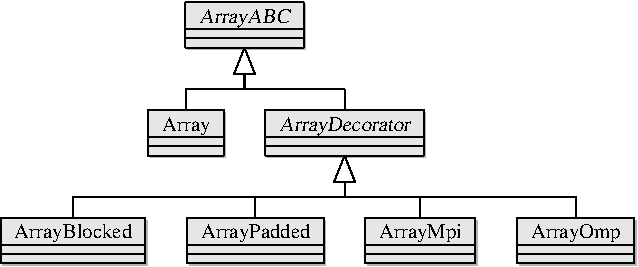
\includegraphics{uml/arrays.1}}

% \centerline{\includegraphics{uml/arrayabc.1}}

\centerline{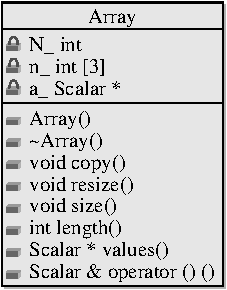
\includegraphics{uml/array.1}}

\subsubsection{Array shape}

\subsubsection{Array blocking}

\subsubsection{Array padding}

\subsubsection{Array interleaving}


\subsection{Attributes}

\begin{tabbing}
xx\=xx\=xxxxxxxxxxxxxxxxxxxxxxxxxxxxxxxxxxx\= \kill
\> \todo \>  \textit{Length of array} \\
\>       \> \code{N\_: int }      \\ \\
\> \todo \>  \textit {Shape of array, right-padded with 1's} \\
\>       \> \code{n\_: int [3] }  \\ \\
\> \todo \>  \textit {Array values stored in column-major ordering}\\
\>       \> \code{a\_: Scalar * }
\end{tabbing}

\subsection{Operations}

\begin{tabbing}
xx\=xx\=xxxxxxxxxxxxxxxxxxxxxxxxxxxxxxxxxxx\= \kill
\> \todo \> \textit{Create a new uninitialized Array object} \\
\>       \> \code{Array()} \\ \\
\> \todo \> \textit{Create a new initialized Array object} \\
\>       \> \code{Array(int n0, int n1=1, int n2=1, int n3=1)} \\ \\
\> \todo \> \textit{Deallocate the array} \\
\>       \> \code{\~{\ }Array()}  \\ \\
\> \todo \> \textit{Copy an array into this one, deallocating any existing data} \\
\>       \> \code{void copy (const Array \&)}  \\ \\
\> \todo \> \textit{Resize the array, deallocating any existing data} \\
\>       \> \code{void resize (int n0, int n1=1, int n2=1, int n3=1)}   \\ \\
\> \todo \> \textit{Return the size of the array} \\
\>       \> \code{void size (int *n0, int *n1=0, int *n2=0, int *n3=0) const}  \\ \\
\> \todo \> \textit{Return the total length of the array} \\
\>       \> \code{int length () const}  \\ \\
\> \todo \> \textit{Return a pointer to the array values} \\
\>       \> \code{Scalar * values () const}  \\ \\
\> \todo \> \textit{Return the given array element} \\
\>       \> \code{Scalar \& operator () (int i0, int i1=0, int i2=0, int i3=0)}
\end{tabbing}

